\chapter{BLAS}
Die Abkürzung BLAS steht für Basic Linear Algebra Subprograms.

\section{Datenstruktur für Matrizen}
Vollbesetzte Matrizen werden bei BLAS entweder zeilen- oder spaltenweise abgespeichert. Das bedeutet, dass entweder die Zeilen- oder die Spalten der Matrix hintereinander im Speicher stehen. 

\begin{align*}
	A=
	\left(\begin{array}{ccc}
	a_{1,1} & a_{1,2} & a_{1,3} \\ 
	a_{2,1} & a_{2,2} & a_{2,3} \\ 
	a_{3,1} & a_{3,2} & a_{3,3} 
	\end{array} \right) \in \mathbb{R}^{m \times n}
\end{align*}
Matrix $A$ Zeilenweise gespeichert\\
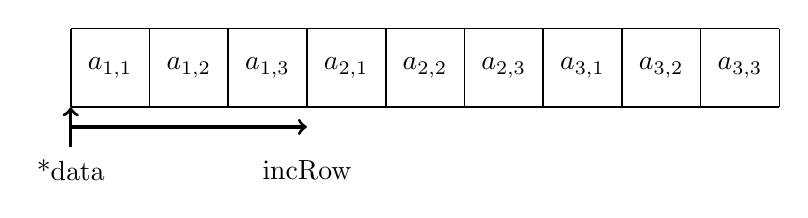
\begin{tikzpicture}
	\draw[semithick] (0,0) -- (9,0);
	\draw[semithick] (0,1) -- (9,1);
	\draw[semithick] (0,0) -- (0,1);
	\draw[semithick] (1,0) -- (1,1);
	\draw[semithick] (2,0) -- (2,1);
	\draw[semithick] (3,0) -- (3,1);
	\draw[semithick] (4,0) -- (4,1);
	\draw[semithick] (5,0) -- (5,1);
	\draw[semithick] (6,0) -- (6,1);
	\draw[semithick] (7,0) -- (7,1);
	\draw[semithick] (8,0) -- (8,1);
	\draw[semithick] (9,0) -- (9,1);
	
	\draw (0.5,0.5) node {$a_{1,1}$};
	\draw (1.5,0.5) node {$a_{1,2}$};
	\draw (2.5,0.5) node {$a_{1,3}$};
	\draw (3.5,0.5) node {$a_{2,1}$};
	\draw (4.5,0.5) node {$a_{2,2}$};
	\draw (5.5,0.5) node {$a_{2,3}$};
	\draw (6.5,0.5) node {$a_{3,1}$};
	\draw (7.5,0.5) node {$a_{3,2}$};
	\draw (8.5,0.5) node {$a_{3,3}$};
	
	\draw[->,line width=0.4mm] (0,-.5) -- (0,0);
	\draw (0,-0.8) node {*data};
	\draw[->,line width=0.4mm] (0,-.25) -- (3,-.25);
	\draw (3,-0.8) node {incRow};
\end{tikzpicture}\\
Matrix $A$ Spaltenweise gespeichert\\
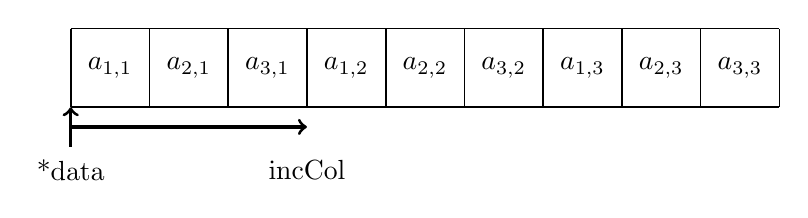
\begin{tikzpicture}
\draw[semithick] (0,0) -- (9,0);
\draw[semithick] (0,1) -- (9,1);
\draw[semithick] (0,0) -- (0,1);
\draw[semithick] (1,0) -- (1,1);
\draw[semithick] (2,0) -- (2,1);
\draw[semithick] (3,0) -- (3,1);
\draw[semithick] (4,0) -- (4,1);
\draw[semithick] (5,0) -- (5,1);
\draw[semithick] (6,0) -- (6,1);
\draw[semithick] (7,0) -- (7,1);
\draw[semithick] (8,0) -- (8,1);
\draw[semithick] (9,0) -- (9,1);

\draw (0.5,0.5) node {$a_{1,1}$};
\draw (1.5,0.5) node {$a_{2,1}$};
\draw (2.5,0.5) node {$a_{3,1}$};
\draw (3.5,0.5) node {$a_{1,2}$};
\draw (4.5,0.5) node {$a_{2,2}$};
\draw (5.5,0.5) node {$a_{3,2}$};
\draw (6.5,0.5) node {$a_{1,3}$};
\draw (7.5,0.5) node {$a_{2,3}$};
\draw (8.5,0.5) node {$a_{3,3}$};
	
\draw[->,line width=0.4mm] (0,-.5) -- (0,0);
\draw (0,-0.8) node {*data};
\draw[->,line width=0.4mm] (0,-.25) -- (3,-.25);
\draw (3,-0.8) node {incCol};
\end{tikzpicture}\\


Eine Datenstruktur benötigt folgende Elemente:
\begin{itemize}
	\item einen Zeiger auf eine Speicherfläche
	\item Informationen ob die Matrix zeilen- oder spaltenweise gespeichert ist 
	\item die Dimension der Matrix.
\end{itemize}


Eine derartige Datenstruktur könnte in C so aussehen.
\begin{lstlisting}
struct Matrix {
  double * data;
  std::ptrdiff_t incRow, incCol;
  std::size_t numRows, numCols;
}
\end{lstlisting}

Für Intel MKL Routinen müssen die Matrizen zeilenweise gespeichert sein.


\section{Einige BLAS-Routinen}
Im Folgenden werden einige BLAS-Routinen beschrieben, die bei der QR-Zerlegung benutzt werden.
BLAS-Routinen werden meist nach folgendem Schema benannt.
Der erste Buchstabe im Namen gibt an für welchen Datentype die Funktion implementiert wurde. Der Rest beschreibt die Funktion der Funktion.\\
Beispiel: \glqq dgemm\grqq{}, das d zeigt an die Funktion ist für Doubles und \glqq gemm\grqq{} steht für \glqq generel Matrix Matrix\grqq{}, die Funktion berechnet also das Matrix-Matrix Produkt für Matrizen deren Einträge Doubles sind.

\subsection{Matrix-Matrix Produkt (gemm)}
Die \glqq gemm\grqq{} Funktion berechnet das Matrix-Matrix Produkt.
Der Funktion werden die Matrizen $A$, $B$ und $C$ und die Skalare $\alpha$ und $\beta$ übergeben. Außerdem werden 2 Flags übergeben ob die Matrizen $A$ und $B$ transponiert werden sollen.\\
Die Funktion berechnet
\begin{align}
	C \leftarrow \beta  C + \alpha  A  B
\end{align}
Falls $\beta = 0$ wird die Matrix $C$ zuerst mit Nullen initialisiert. Falls $C$ Einträge hat die NaN (Not a Number) sind, werden diese somit mit 0 überschrieben.

%%TODO
Blas tecnicla forum netlib
%%http://www.netlib.org/blas/blast-forum/

\subsection{Matrix-Vector Produkt (gemv)}
Die Funktion \glqq gemv\grqq{} berechnet das Matrix-Vector Produkt.
Der Funktion wird die Matrix $A$ die Vektoren $x$ und $y$ und die Skalare $\alpha$ und $\beta$ übergeben. Außerdem wird ein Flag übergeben das anzeigt ob die Matrixa Transponiert werden soll.\\
Die Funktion berechnet
\begin{align}
	y \leftarrow \beta  y + \alpha A x 
\end{align}
Falls $\beta = 0$ wird der Vektor $y$ zuerst mit Nullen initialisiert. Falls $y$ Einträge hat die NaN (Not a Number) sind, werden diese somit mit 0 überschrieben.
\subsection{Rank1 update (ger)}
Die Funktion \glqq ger\grqq{}  berechnet ein dyadische Produkt aus den Vektoren $x$ und $y$, skaliert die daraus resultierende Matrix mit $\alpha$ und addiert das Ergebnis auf $A$.//
Der Funktion wird die Matrix $A$ die Vektoren $x$ und $y$ und das Skalar $\alpha$ übergeben.\\
Die Funktion berechnet
\begin{align}
	A \leftarrow A + \alpha  x y^T
\end{align}

\subsection{Matrix-Matrix Produkt (trmm)}
Die Funktion \glqq trmm\grqq{} berechnet das Matrix-Matrix Produkt einer Dreiecksmatrix mit einer voll besetzten Matrix.
Der Funktion wird die Dreiecksmatrix $A$, die Matrix $B$ und das Skalar $\alpha$ übergeben. Außerdem werden Flags mit übergeben die anzeigen ob $A$ eine obere oder unter Dreiecksmatrix ist, ob $A$ eine strikte oder unipotente Dreiecksmatrix ist, ob $A$ von links oder rechts auf $B$ multipliziert werden soll und ob $A$ transponiert werden soll.
%% TODO stimmt unipotente Dreiecksmatrix?
\\
Die Funktion berechnet
\begin{align}
B \leftarrow  \alpha \cdot op(A) \cdot B \qquad \text{or} \qquad B \leftarrow  \alpha \cdot B \cdot op(A)
\end{align}
\subsection{Matrix-Vector Produkt (trmv)}
Die Funktion berechnet das Matrix-Vector Produkt für Dreiecksmatrizen.
Die Funktion berechnet
\begin{align}
x \leftarrow \alpha  Ax %\qquad \text{or} \qquad x \leftarrow \alpha * A^T*x
\end{align}

